\section{Results \& Discussion}\label{sec:results}

\subsection{Fitting Sorption Parameters}\label{sec:results_sorption_fit}

Using the numerical fitting scheme described in section \ref{sec:indoor_environment} with the sorption data from the method described in section \ref{sec:experimental_method}, the kinetic sorption parameters $k_1$ and $k_2$ are determined.
Figure \ref{fig:sorption_fit} shows the result of this fitting and the sorption data for three select materials - wood, Appling soil, and cinderblock concrete.
The $k_1$ and $k_2$ represent the rate at which TCE desorbs and sorbs respectively onto/from the material of interest.
The equilibrium sorption constant is, using the formulation in \eqref{eq:sorption_rate}, given by
\begin{equation}
  K = \frac{k_1}{k_2}
\end{equation}
and is used as the sorption isotherm.
Here a small $K$ indicate that there is a greater propensity for contaminant sorption.\par

To use the soil sorption isotherm in \eqref{eq:mass_transport} $K$ needs to be converted from being unitless to $\mathrm{m^3/kg}$.
This is done by multiplying the inverse of $K$ isotherm with inverse of the soil bulk density $\rho_b$, which is taken to be $1460 \; \mathrm{kg/m^3}$.
\begin{equation}
  K_\mathrm{ads} = \frac{1}{K \rho_b} = 5.28 \; \mathrm{(m^3/kg)}
\end{equation}

\begin{figure}[htb!]
  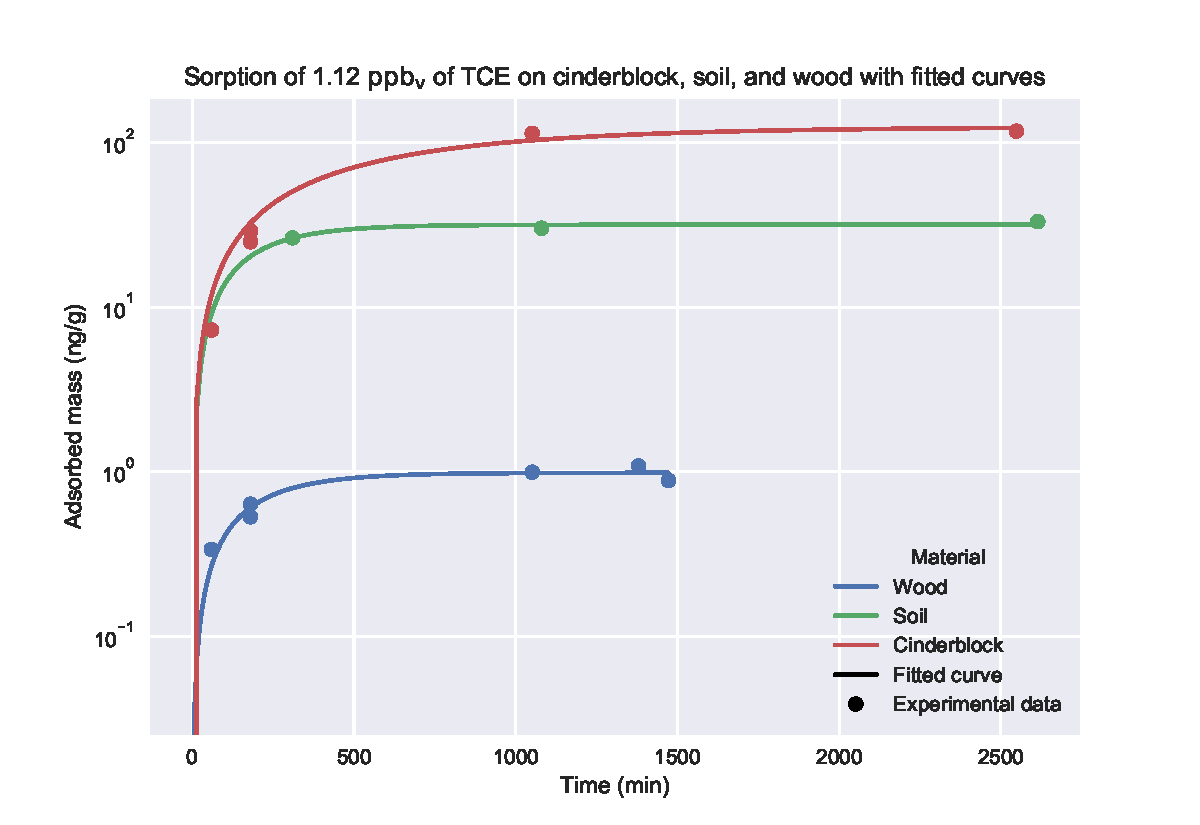
\includegraphics[width=\textwidth]{sorption_fit.pdf}
  \caption{Experimental data of sorption of TCE onto three select materials as well as fitted sorption rates based on the kinetic model \eqref{eq:sorption_rate}.}
  \label{fig:sorption_fit}
\end{figure}

% TODO: Shuai: Some thoughts or comments about these values? I.e. why is cinderblock so much larger?
Table \ref{tbl:sorption_fit} shows the fitted parameters for the tested materials.
Based on this these results we can see that cinderblock and soil have orders of magnitude larger sorption capacities than wood or drywall does.
We can also see by the $k_2$ values that soil and cinderblock sorb quickly, much faster than a material with similar sorptive capacity such as paper.\par
\textit{Note: Here I envision some explanation/discussion on why there is a such a big difference in sorptive capacities. I've asked Shuai to write about this.}

% TODO: Add the relative sorbed mass compared to air. I.e. cinderblock has ~ 7800 more mass for the same volume.
\begin{table}[htb!]
  \caption{Fitted kinetic sorption parameters based on sorption experiment data. Six different types of materials are considered. $k_1$ and $k_2$ are the desorption and sorption constants respectively, and $K$ is the sorption equilibrium constant.}
  \label{tbl:sorption_fit}
  \centering
  \begin{tabular}{l c c c}
    \toprule
    Material & $k_1 \; \mathrm{(1/hr)}$ & $k_2 \; \mathrm{(1/hr)}$ & $K$ \\
    \hline
    Wood & 0.32 & 44.90 & $7.10 \cdot 10^{-3}$ \\
    Drywall & 0.41 & 87.94 & $4.65 \cdot 10^{-3}$ \\
    Carpet & 0.26 & 58.74 & $4.42 \cdot 10^{-3}$ \\
    Paper & 0.04 & 88.37 & $4.55 \cdot 10^{-4}$ \\
    Soil & 0.34 & 2636.57 & $1.30 \cdot 10^{-4}$ \\
    Cinderblock & 0.10 & 4175.16 & $2.40 \cdot 10^{-5}$ \\
    \bottomrule
  \end{tabular}
\end{table}

\subsection{Soil Sorption's Retarding Effect}\label{sec:retardation_effect}

Building pressurization is a key factor in VI that influences the advective contaminant transport.
The magnitude of change in response to a pressurization change is significantly influenced by a range of factors, such as soil permeability, foundation depth, or soil moisture, and of course - sorption, which we will focus on.
To investigate the effect that soil sorption has on contaminant soil mass transport in the VI context, we run two types transient simulation where initially the modeled structure is depressurized at a steady -5 Pa.
At the start of the simulation, the building building is further depressurized to -15 Pa \eqref{eq:equilibrium_depressurization}, or overpressurized to 15 Pa \eqref{eq:equilibrium_overpressurization}, and the simulation is allowed to run for 72 hours. % TODO: Update this once the new simulations are done.
\begin{align}
  \text{Depressurization}: \; \Delta p_\mathrm{in/out} &= \begin{cases}
    -5, \; &t = 0 \; \mathrm{(hr)} \\
    -15, \; &0 < t \leq 72 \; \mathrm{(hr)}
\end{cases}\label{eq:equilibrium_depressurization}\\
\text{Overpressurzation}: \; \Delta p_\mathrm{in/out} &= \begin{cases}
  -5, \; &t = 0 \; \mathrm{(hr)} \\
  15, \; &0 < t \leq 72 \; \mathrm{(hr)}
\end{cases}\label{eq:equilibrium_overpressurization}
\end{align}
For each of these cases, the simulation is run using two different soil types - sand and sandy loam.
Sand is assumed here to not sorb any TCE, while for sandy loam a range of sorption isotherms are used.
These range from no sorption ($K_\mathrm{ads} = 0 \; \mathrm{(m^3/kg)}$) to the experimentally determined sorption isotherm ($K_\mathrm{ads} = 5.28 \; \mathrm{(m^3/kg)}$) in intervals multiplicative by $10^{-2}$. With the experimentally determined isotherm, we see that the ratio between sorbed concentration and soil-gas phase concentration is 7708, i.e. there is a much larger amount of sorbed contaminant.
When $K_\mathrm{ads} = 5.28 \cdot 10^{-4} \; \mathrm{(m^3/kg)}$ this ratio is roughly unity (0.77), which is good to keep in mind in the following discussion. % TODO: Make sure you change this value if you rerun the simulation later with a different H
These ranges of values can be used both to represent a soil that has a smaller sorptive capacity or a situation where the sorbed and gas phase has not quite reached equilibrium.\par

\begin{figure}[!htb]
  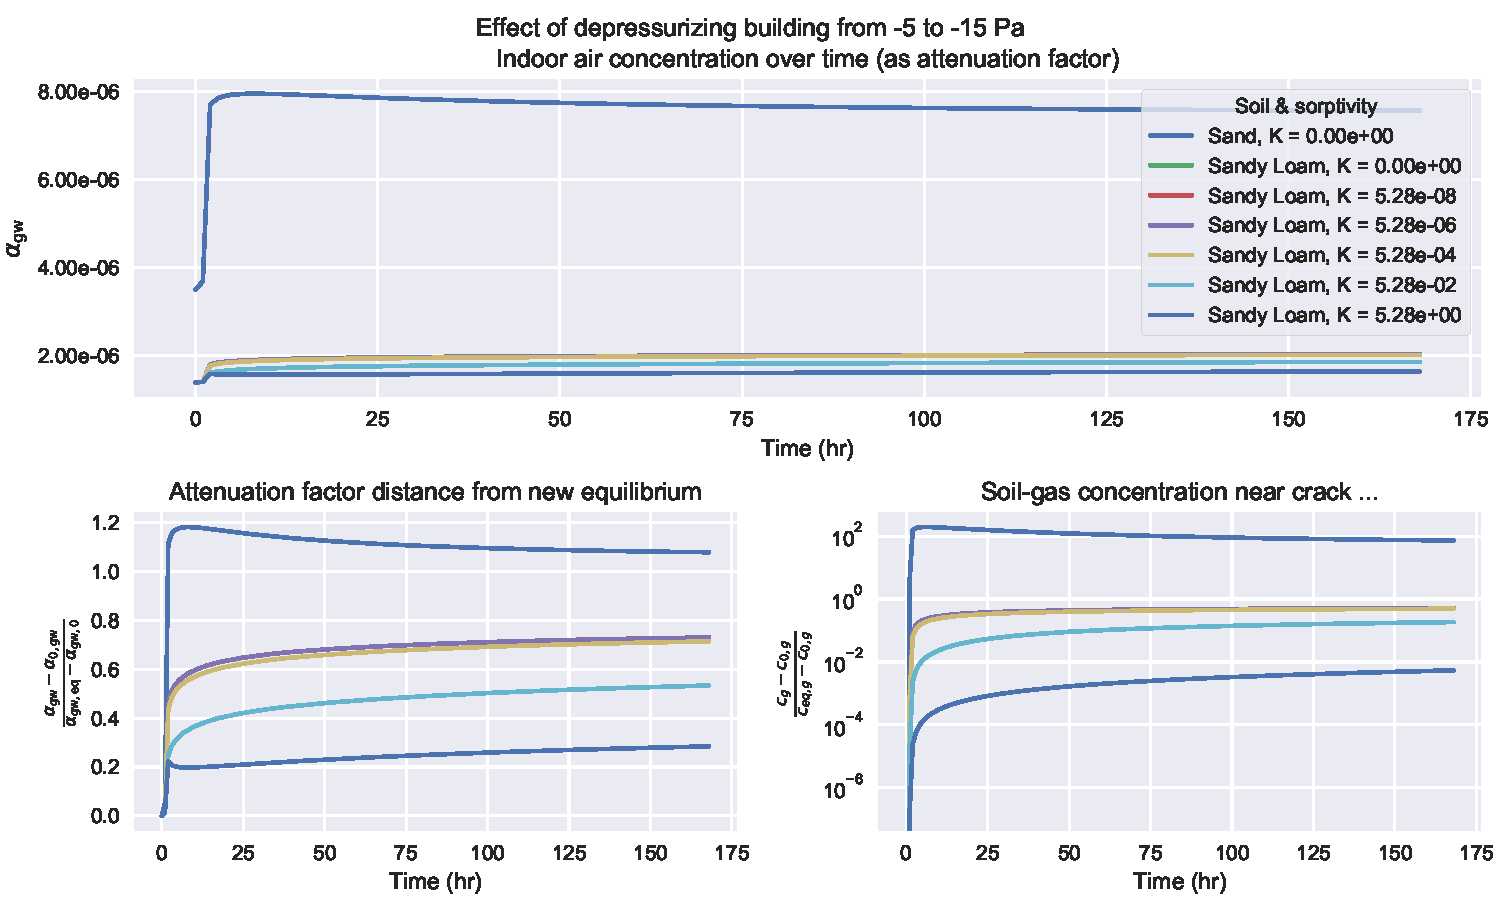
\includegraphics[width=\textwidth]{equilibrium_retardation_depressurization.pdf}
  \caption{}
  \label{fig:equilibrium_depressurization}
\end{figure}

The top panel of Figure \ref{fig:equilibrium_depressurization} shows the indoor air contaminant concentration as the simulated building is undergoing the pressurization in \eqref{eq:equilibrium_depressurization} case.
Here we can see that for the when the surrounding soil consists of sand, the indoor concentration increases rapidly as the building is further pressurized.
The rate of increase decreases significantly for the sandy loam cases, and progressively retards are the sorbed mass increases ($K_\mathrm{ads}$ increases).\par

The bottom left panel shows how far away the indoor air concentration (as attentuation factor) for each case is from reaching equilibrium.
At the start of the simulation, the building starts with an attenuation of $\alpha_0$, which is the steady-state concentration when the building is pressurized with -5 Pa.
As the building is further depressurized to -15 Pa, the indoor air concentration will approach a new equilibrium state $\alpha_{eq}$ (the result of which is from a steady-state simulation at that pressurization).
By plotting $\frac{|\alpha-\alpha_0|}{|\alpha_{eq}-\alpha_0|}$ we can easily see how far away we are from the new equilibrium state, and a value of 0 represents that we are at the initial concentration, i.e. $\alpha = \alpha_0$, and a value of 1 represents $\alpha = \alpha_{eq}$, i.e. that the new equilibrium has been reached.\par

This sort of analysis is applied to the bottom right panel as well, but instead of the indoor air concentration (as attentuation factor), we consider the average soil-gas concentration in a 5 cm diameter cylinder that envelop the entire perimeter crack.
The choice of 5 cm is arbitrary, but helps illustrate what happens in the near-foundation-crack region soil-gas concentration, changes in which allow us to better understand how the contaminant is transported into the building from the soil.
The same could be done for the soil-gas velocity of course, but the rate of soil-gas velocity change is virtually the same for all of these cases, and reaches the new equilibrium velocity very quickly (much faster than the concentration) and is thus omitted from the figure.\par

Before discussing the role of sorption here, we can first compare the non-sorbing sand and sandy loam cases.
Due to the higher permeability and lower moisture content, sand is significantly more permeable to gas flow than sandy loam (see Table \ref{tbl:model} for permeability values).
Consequently the advective transport through the foundation crack is much more significant, which is indicated by a Péclet number of around 4 versus 0.2 at a -15 Pa pressurization for sand and sandy loam respectively.\par

Due to the advection dominated transport mechanism in the sand case, the indoor air concentrations are temporarily elevated above the equilibrium concentration at -15 Pa, while the soil-gas concentration moves further away from equilibrium.
(Note that the absolute distance from equilibrium is plotted in Figure \ref{fig:equilibrium_depressurization} which is why at first glance one might think that the soil-gas concentration is two order of magnitude higher initially, but actually is two order of magnitude lower.)
This phenomena occurs because initially more contaminants are drawn into the building from the near crack area than can be resupplied, temporarily depleting the local soil-gas contaminant concentration.\par

One can notice that many of the sandy loam lines overlap, and start diverging from each other when $K_\mathrm{ads} = 5.28 \cdot 10^{-4} \; \mathrm{(m^3/kg)}$, at the point where the ratio of sorbed and soil-gas concentration are roughly equal.
We see that this divergence occurs simultaneously in the indoor air and soil-gas contaminant concentration.
However, since the indoor air concentration depend on the soil-gas concentration, we know that this is where the relevant difference is.\par

The simple reason for this is that it is at this threshold the sorptive contribution to the retardation factor \eqref{eq:retardation_factor} starts to becomes larger than the other terms.
\begin{equation}
   \rho_b K_H K_\mathrm{ads} > \theta_w + \theta_g K_H
\end{equation}
Thus it is at this point that the contaminant transport in the soil starts to become retarded by sorption.
The physical reason for this is that the partitioning between the various phases gives a residence time as the contaminant is transported.
Under VI conditions, the values of $\theta_w + \theta_g K_H$ are bounded to relatively small values, while $K_\mathrm{ads}$ can vary by orders of magnitude, making sorption potentially a very significant retarder for soil transport.\par

We can also note that the retarding effect of sorption also somewhat depends on the contaminants Henry's Law constant $K_H$, bulk density $\rho_b$ and the moisture content $\theta_w$.
For instance if the ambient temperature is higher, then contaminant $K_H$ is likewise larger, and sorption induced retardation is greater.
Generalizing this is difficult however, as $K_\mathrm{ads}$ is also temperature dependent, and the interplay between these may be complicated.
Nevertheless this hints that there may be a climate/weather component to how significantly sorption induced retardation is.\par

Figure \ref{fig:equilibrium_overpressurization} shows the same sort of analysis as in Figure \ref{fig:equilibrium_depressurization} but with the building pressurization following \eqref{eq:equilibrium_overpressurization}.
The results here are more or less the same, with the notable exception that in the sand case, the final equilibrium concentration is not initially exceeded.
As the building is overpressurized, the indoor contaminant are pushed out into the soil.
Since the indoor air concentration is lower than the soil-gas concentration, this is entirely expected.\par

\begin{figure}[!htb]
  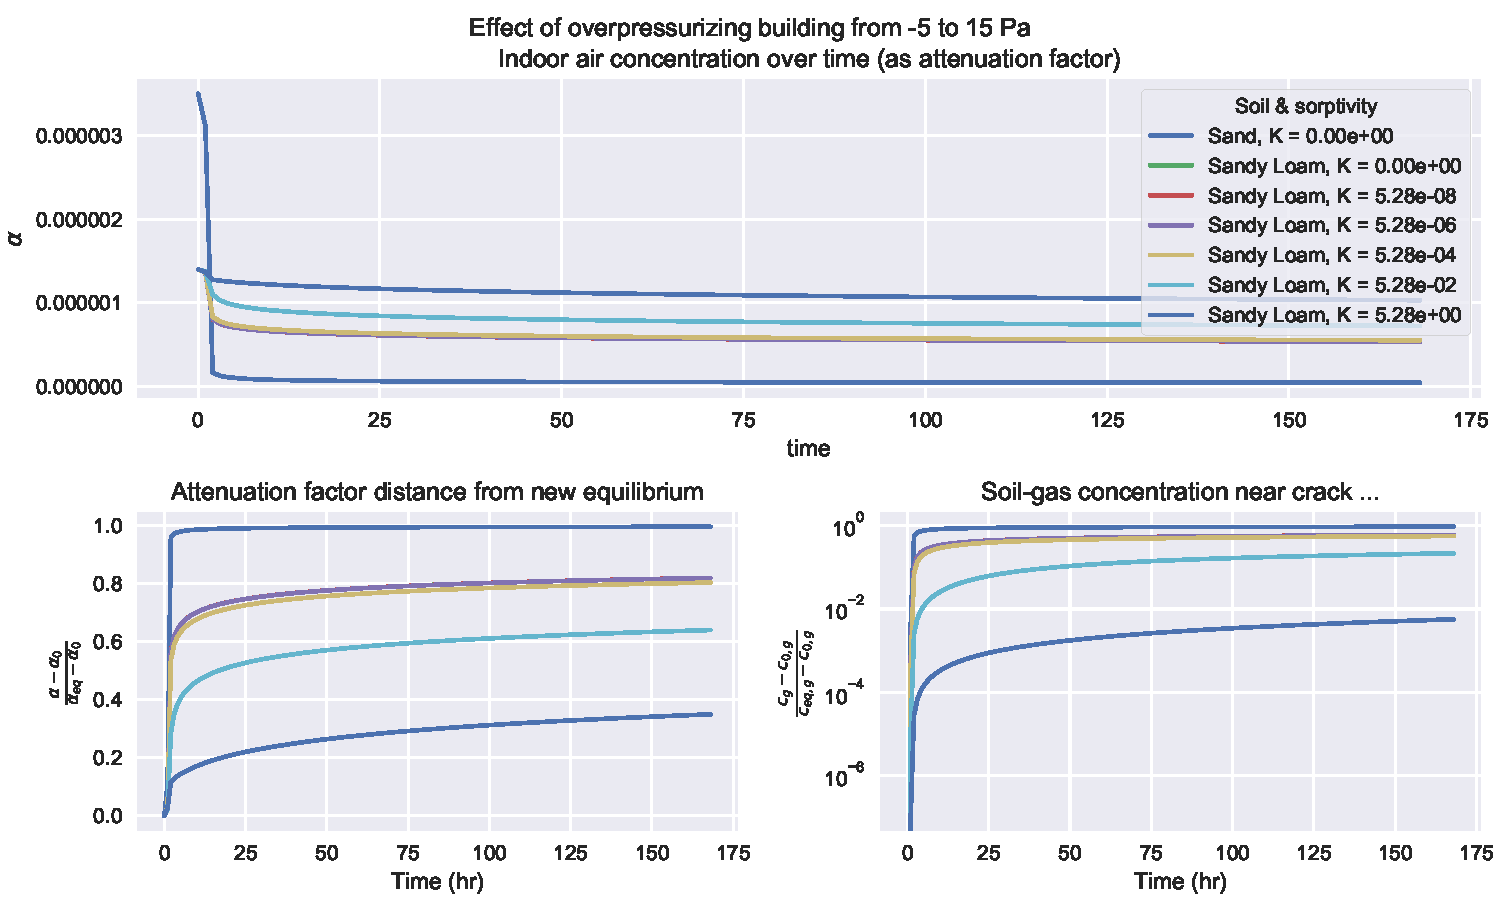
\includegraphics[width=\textwidth]{equilibrium_retardation_overpressurization.pdf}
  \caption{}
  \label{fig:equilibrium_overpressurization}
\end{figure}

% TODO: Some concluding remarks or keep this solely for the conclusion section?

\subsection{Indoor Material Sorption And Dynamics}\label{sec:results_indoor_sorption}

Now we turn to exploring the effect of sorption onto/from various indoor materials has on the indoor air contaminant concentration, again through our model.
For these simulations we assume that there is no soil sorption.
To study this we consider the basement (the indoor air space) and assume that the inside surfaces are entirely made up of one of the materials we studied in \ref{sec:results_sorption_fit}.
We also assume that the material covering the indoor surfaces has a certain thickness or depth that the contaminants can penetrate - giving a certain volume or mass of sorbing material in the indoor.
Table \ref{tbl:sorbed_material} shows the surface area, penetration depth, and volume of each material studied.
While obviously some of these rooms are non-conventional and arbitrarily designed, i.e. you're unlikely to find a room with carpeted walls, floors, and ceiling, they do present some limiting cases of the potential effect of sorption onto/from these materials.\par

% TODO: Do I want to include some more information/data here? Sorbed mass at t0?
\begin{table}[htb!]
  \centering
  \begin{tabular}{l c c}
    \toprule
    Material & $d_\mathrm{p} \; \mathrm{(mm)}$ & $V_\mathrm{mat} \; \mathrm{(m^3)}$ \\
    \hline
    Cinderblock & 5 & 1.6 \\
    Wood & 1 & 0.32 \\
    Drywall & 10 & 3.2 \\
    Carpet & 10 & 3.2 \\
    Paper & 0.1 & 0.032 \\
    \bottomrule
  \end{tabular}
  \caption{The assumed contaminant penetration depth and subsequent volume of the sorbing indoor materials. The material surface area is assumed to be the same, and each material completely cover the surfaces of a 10x10x3 meter room.}
  \label{tbl:sorbed_material}
\end{table}

The modeled building then undergoes a pressurization cycle, where at start of the simulation it is depressurized at -5 Pa and at steady-state.
The building is then sequentially depressurized to -15 Pa, then pressurized to 15 Pa, and finally again depressurized to -5 Pa.
For each sequence, the new pressurization is maintained for 24 hours.
This pressurization cycle may be seen in the top left panel of \ref{fig:indoor_sorption_cycle}.
The choice of pressurization cycle is somewhat arbitrary, but ours can be used to represent limiting cases of natural pressurization variation, or artificially induced pressurization.
Figure \ref{fig:indoor_sorption_cycle} shows the result of these simulations.\par

The change in indoor air contaminant concentration over this pressurization cycle is shown in the bottom panel of Figure \ref{fig:indoor_sorption_cycle}.
First we consider the reference case - where there is no sorbing indoor materials present.
(The blue line is the reference case, which may be difficult to see as the wood and carpet lines overlap.)
Here we see that as the building is depressurized, the indoor air contaminant concentration increases quickly in response to the pressurization change, and is approaching an equilibrium.\par

% TODO: Plot the sorption rate r normalised to the entry rate n_ck? Should be ~1 when materials becomes saturated. Nice way to non-dimensionalize this too. Maybe as second axis plot on the top right panel?
\begin{figure}[!htb]
  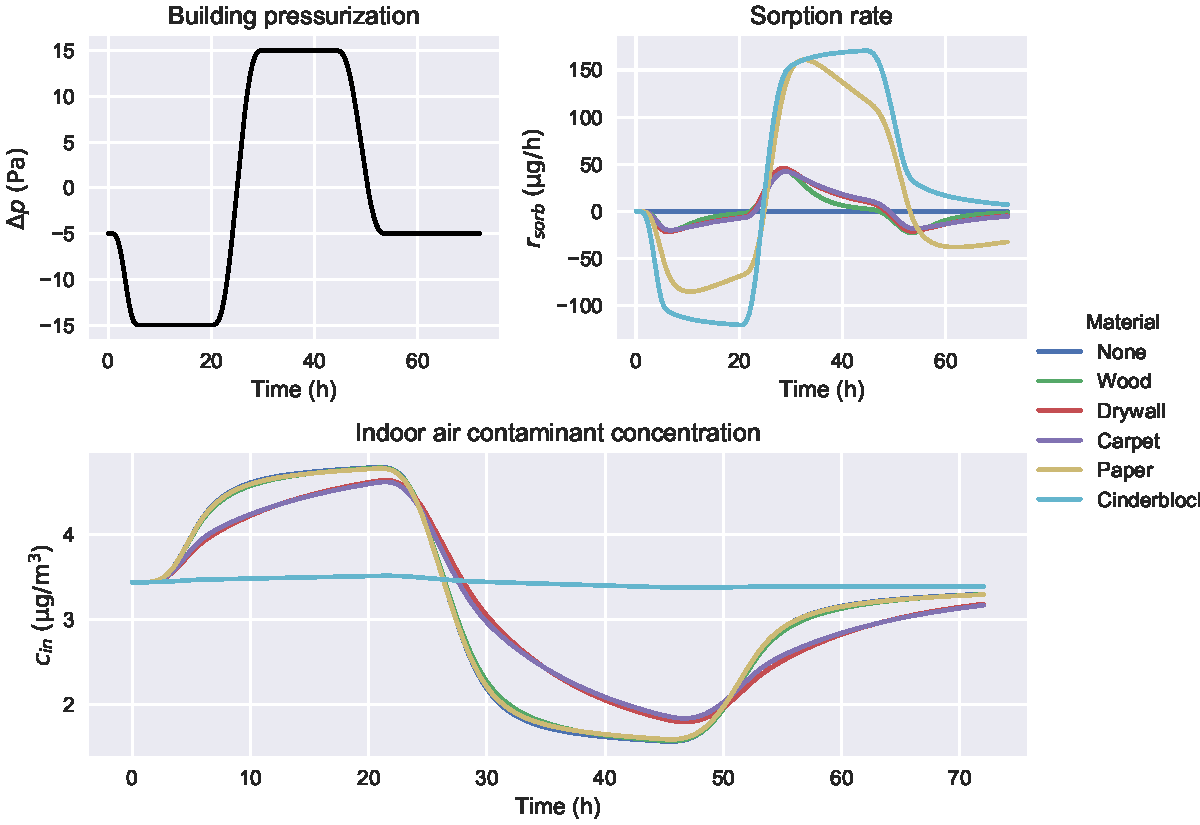
\includegraphics[width=\textwidth]{sorption_indoor_cycle.pdf}
  \caption{
  Comparison of how sorption onto/from various indoor materials affect the indoor air contaminant concentration (bottom) of a building that undergoes a pressurization cycle (top left). The rate of de- and sorption for each considered material during the cycle are also shown (top right) and is governed by \eqref{eq:sorption_rate}. A positive value means that contaminant vapors are being sorbed onto/into the material and a negative means the material is desorbing into the indoor air space.}
  \label{fig:indoor_sorption_cycle}
\end{figure}

By observation we can see that the presence of the various studied building materials in the indoor environment has a very different effect on the change in indoor air contaminant concentration.
The presence of wood and carpet has close to no effect on the indoor air concentration.
While cinderblock has a very significant effect, preventing almost any change in indoor concentration.
Drywall and carpet is in the middle significantly delays the rate of change in the indoor concentration, but for each 24 hour cycle, roughly the same indoor concentration is reached as the reference case.\par

The disparity of these result is explained by the the top right panel of Figure \ref{fig:indoor_sorption_cycle}.
Here the de- and sorption rates in $\mathrm{\mu g/hr}$ for each considered indoor material is shown.
A positive and negative value here indicate that contaminant is desorbed respectively sorbed to and from the material.
To understand this figure, it is useful to refer back to Table \ref{tbl:sorption_fit} which show the sorption and desorption rate constant $k_1$ and $k_2$ respectively, and the sorption equilibrium constant $K$ (a smaller value indicate a larger sorptive capacity).\par

First we consider to the depressurization part of the cycle (1-25 hours).
(Here see that the reference case has no sorption at all, by definition.)
And similar to the indoor concentration panel, we see that the wood, drywall, and carpet cases overlap.
This is explained by these materials have similar sorptive capacities ($K$) and sorptive rates ($k_2$).
Paper by contrast has a similar shape to the three previously mentioned, while the magnitude is significantly larger.
This is because the $K$ value for paper is one order of magnitude larger, indicating that wood, drywall, and carpet saturate with contaminant vapors over the time period, while paper does not.
Cinderblock has a further order of magnitude larger $K$ value, thus is even further away from being saturated, which explains the even faster sorption rate.\par

Next we consider the overpressurzation period (25-49 hours).
Again we see here that wood, drywall, and carpet behave the similarly for the same reasons as before, i.e. the desorption rate constants $k_1$ and sorption equilibrium constants $K$ are similar.
This means that these reach the new sorbed contaminant saturation at roughly the same time.\par

Here it is important to note that due to the diffusion dominated transport through the foundation crack, even though the building is overpressurized, there is substantial contaminant entry.
And because the sole contaminant source is the modeled contaminated groundwater, the sorbed equilibrium is relative to this entry rate.\par

Paper and cinderblock initially behave very similarly during the overpressurization period and desorb contaminants quickly.
However, paper reaches its saturation limit after a relatively short time, while cinderblock has not even at the end of the overpressurization cycle.
Since the desorption rate constants $k_2$ are relatively similar for the materials, thus this disparity is primarily due to the different sorption equilibrium constants $K$.\par

Lastly, we consider the final period where the pressurization goes back to its initial state (49-72 hrs).
Here we see that the reference case does not quite return to the initial indoor concentration.
Thus the contaminant entry rate has not equilibrated yet, due to the soil contaminant concentration has not done so either.
Like in the previous analysis we again see that the wood, drywall, and carpet cases don't differ from the reference.
The paper case is slightly more different, but for the same reasons that have already been discused.
Cinderblock is unique here though, as we clearly see that it is releasing contaminants, due to the previous change in contaminant concentration has been so significantly retarded.\par


From this simulation work we can see how varied the effect of sorbing indoor materials are.
Most of the tested materials only have a moderate effect on the indoor air contaminant concentration dynamics, with the notable exception of cinderblock, which effectively enforces as pseudo-steady-state.
However we also see from the analysis of the sorption dynamics that the de- and sorption rate constants $k_1$ and $k_2$ are less important than the sorptive capacity $K$ of the material.\par

\subsection{Indoor Material Sorption And Mitigation}\label{sec:results_indoor_mitigation}

The work done by us and others have shown the large sorptive capacities of various common materials.
The desorption of the sorbed contaminants may have significant impact on the efficacy of various mitigation systems.
To investigate this we turn to our model and consider a scenario where initially the modeled building is depressurized with -5 Pa and at the start of the simulation some perfect mitigation scheme is  turned on and the contaminant entry $n_\mathrm{entry}$ in \eqref{eq:cstr} goes to zero.
We also assume that for each case, the indoor environment contains the same amount of indoor material as described in section \ref{sec:results_indoor_sorption}.
The air exchange rate is assumed to remain a constant 0.5 per hour for the entire 72 hour simulation time.\par % TODO: Update this time if you run a longer simulation later.

The decrease in indoor air concentration (as attenuation factor $\alpha$) for each simulated case is seen in Figure \ref{fig:sorption_mitigation}.
As excepted, when there is no sorbing indoor materials, i.e. our reference case, the indoor concentration decreases log-linearily.
We can also see that the contaminant desorption from the materials maintain a higher indoor air concentration relative to reference, with cinderblock again shown to have the great impact.\par

\begin{figure}[!htb]
  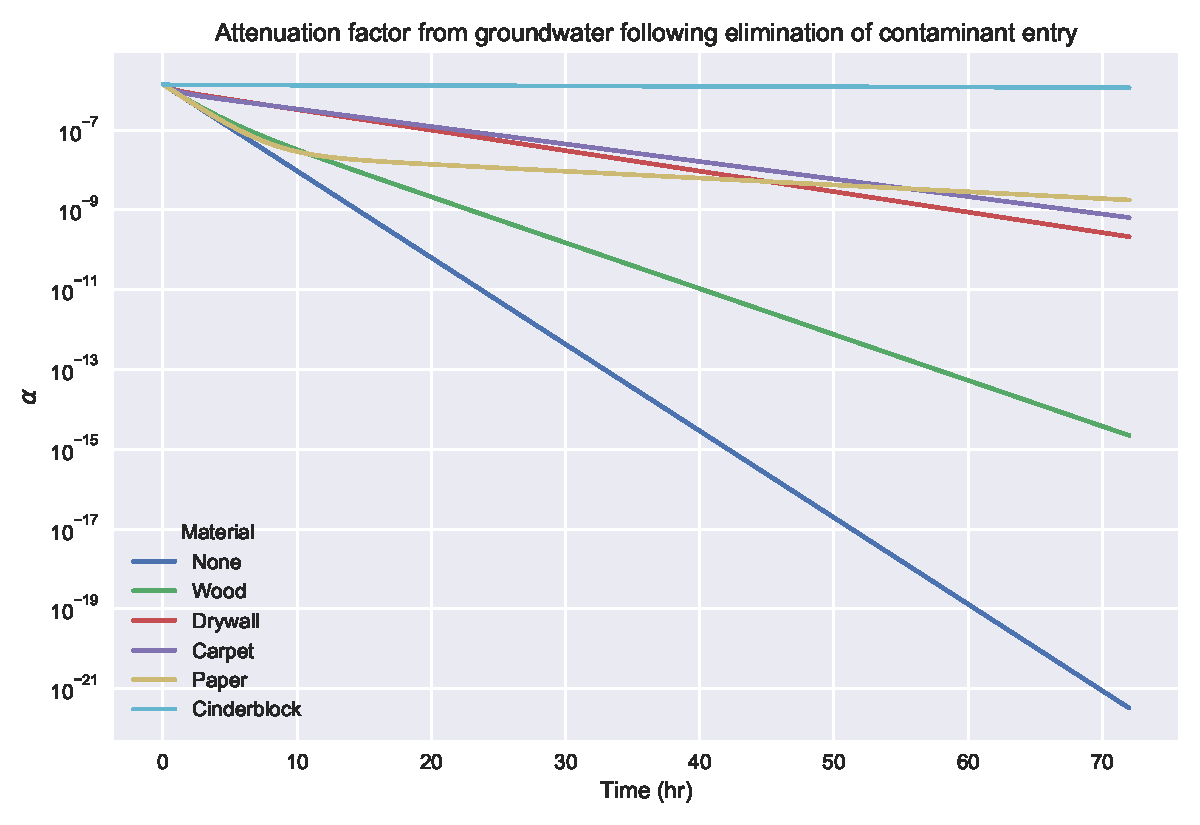
\includegraphics[width=\textwidth]{sorption_mitigation.pdf}
  \caption{}
  \label{fig:sorption_mitigation}
\end{figure}

\textit{Note that this section is still incomplete as I am still working on expanding/improving the analysis/figure.}
